   
\section{Methodology}
\subsection{Data Imbalance}

The initial issue faced when starting to attempt to build a prediction model was how to split the continuous variables supplied by the EmoBank dataset into discrete categories.

The decision to split the data into discrete categories was done since it is easier to utilise classification methods produced by previous work as they tend to use discrete classes like Positive, Neutral and Negative to represent sentiment. The output data for each V,A,D value will be defined as one of a set number of classes, the same number of classes as the input.

To discover the optimal way that the data can be split, the imbalance created over the dataset when the the classes are created in different ways will be analysed and compared. The imbalance over the data should ideally be as low as possible.

\subsection{Hypothesis Tests}

To argue for each of the decisions made when building the final model, a hypothesis test with a 95\% confidence level will be carried out.

Due to the imbalance in the data, a prediction accuracy cannot be used for comparing the models. This is because the majority class dominates, with it being the most likely to be predicted as there are simply more examples available \cite{al2015applied}, heavily biasing the accuracy results.

For each investigation that is carried out, a confusion matrix is be produced as shown in Table \ref{conmat}, so that proper analysis of the results can be made.

\begin{table}
\centering
\begin{tabular}{|p{3cm}|p{3cm}|p{3cm}|p{3cm}|p{3cm}|}
 \hline
  & \multicolumn{3}{|c|}{Predicted} & \\
 \hline
   Actual & Negative & Neutral & Positive & \\
    \hline
    Negative &  True Negative   &  False Negative  & False Negative & Total Negative \\
    Neutral & False Neutral & True Neutral&  False Neutral & Total Neutral \\
    Positive & False Positive & False Positive &  True Positive & Total Positive \\
    \hline
    & Total Predicted Negative & Total Predicted Neutral & Total Predicted Positive & \\
 \hline
\end{tabular}
\caption{Structure of produced confusion matrices}
\label{conmat}
\end{table}

The F1 score of the prediction model is used in the hypothesis tests. The F1 score for a defined class is the weighted average of the Precision and Recall for that class in a model, which is defined as follows: 

$$ F1_{Class} = 2 * \frac{Precision_{Class} * Recall_{Class}}{Precision_{Class} + Recall_{Class}} $$

And then the precision and recall values can be calculated as follows, calculated from the confusion matrix given in Table \ref{conmat}.
For example for the Negative class:

$$ Precision_{Negative} = \frac{\textnormal{True Negative}}{\textnormal{Total Predicted Negative}} $$

$$ Recall_{Negative} = \frac{\textnormal{True Negative}}{\textnormal{Total Negative}} $$

It follows for the other two classes in this aspect in the same format.

Each of the experiments are run with stratified K-Fold validation, with the data from each fold being used for the hypothesis test comparisons, using 10 folds. The folds are stratified so that the representation of each class remains the same in each fold which is needed due to the large data imbalance \cite{kohavi1995study}.

Using this score instead of the accuracy gets rid of the class bias, and in this case it is calculated using the micro-average of the K-Folds. The micro average aggregates the contributions of each class so that any imbalance can be mitigated.

The hypothesis test that will be performed on the data will be the Wilcoxon Signed-Rank Test, since the comparison between the data will be on two related samples, and the data cannot be assumed to be normally distributed within the folds, meaning that this is the best test to be using in this case \cite{wilcoxon1970critical}.

\subsection{Lexicon Analysis}

For the bag-of-words model, we will calculate the confusion matrix and then the F1 score by totalling up the values for each sentence over the Emobank dataset, and then comparing the two results, the calculated values, and the ones given in Emobank sample. The values are calculated by looking up each word in the bag-of-words dataset \cite{wordsData}.

To get the words from the EmoBank dataset into a state where they are most likely to be found within the lexicon database, some natural language processing needs to be done on the data, using the NLTK \cite{NLTKBook} library to stem the words, returning words to their root form.

For example, the word "Fishing" would be reduced to the word "Fish" after being stemmed. 

As we can see from Figure \ref{lexiconGraph}, the average values for the Arousal are much lower across the bag-of-word dataset than the average values for the Valence or the Dominance, which may have an effect on the output results since the three dimensions in the EmoBank dataset have similar average values as shown in Figure \ref{dist:vad}.


\subsection{Data Pre-processing (N-Gram and Feature selection)}

Following R. Kim's investigations into semantic analysis \cite{towardsDS}, an investigation into optimising the format for the data input is carried out. 

To be able to analyse the text, the sklearn CountVectorizer library is used to return a sparse matrix of the counts of each word in the input vocabulary, which then become the features for inputting into a machine learning classifier \cite{sklearn}.

From this we can also limit the number of features that we can take, with the number of features being the number of most popular N-Grams, and we can set the N-Gram range easily. 

The previous investigation only tried N-Gram values ranging up to trigram, but to ensure that this is an optimal result, the experiment will be carried out up to fourgram.

The range of features that was used previously was up to 10,0000 features because the results did not improve after this, but since we are using a different dataset, the number of features tested was increased until the resultant graph implied that the F1 score did not improve further. 

The model used to investigate how the F1 score varies as the inputs change will be a Logistic Regression model, as this has been shown to give the most promising results in previous work \cite{towardsDS}.

\subsection{Model Selection}

To choose the models to compare, we will take the top models compared in previous sentiment analysis work \cite{towardsDS} and see which can work best in this situation. \todo{expand on this}

\subsection{Oversampling and Undersampling}

To carry out the investigation of applying the oversampling and undersampling methods, the library functions in the imblearn API is used, which can be used in conjunction with the sklearn methods easily. 

Since it is unclear whether these methods will actually improve the model, comparing against the model that we already have is necessary.

\todo{also expand on this}

\subsection{Implementation}

In terms of developing the sentiment analysis tool, using Python is a clear choice due to the number of Natural Language Processing (NLP) and machine learning libraries available. The main library that will be utilised is the sklearn library \cite{sklearn}, as it has many in-built machine learning classifiers that can be implemented easily, and there is plenty of documentation to support development with this. 

Using other libraries such as Tensorflow is also applicable in this case,  and they are a powerful tool for building models that utilise neural networks, but in this case using the "off-the-shelf" classifiers given by the sklearn library is all we need for this investigation.

The simplest solution to provide an interface between the final produced semantic prediction model and the Spotify API is to create a web application. \todo{talk about the spotify API} The final classification model was hosted on a very simple python server that takes text as an input, and returns whether it classes the text as Positive, Negative or Neutral for each of the Valence, Arousal or Dominance dimensions. 

The final solution, as shown in Figure \ref{implementationLayout}, consists of three distinct hosted solutions, two of which access the API hosted by Spotify to access song data and authentication the user to allow their top songs to be obtained.

The UI was chosen to be built in Angular.js and the music API with Node.js due to prior development knowledge, and hence ease of prototyping. 
To ensure that any resultant song given back was one that the user could relate to, the final song is taken from a selection of the users recent top songs, which they allow the application access to through the authentication process.
The music API, built in Node.js is influenced by the structure of existing Spotify API projects \cite{moodtape}, and is built mostly using the Node package spotify-web-api-node \cite{nodeSpotify}.

\begin{figure}[ht]
\caption{General layout of how the web application should be structured.}
\centering
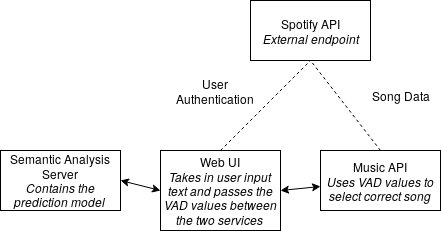
\includegraphics[scale=0.6]{litImgs/interfaceLayout.png}
\label{implementationLayout}
\end{figure}

Choosing how to relate the VAD values to the data returned for the songs is relatively arbitrary,and something that if there was more time could be investigated further. Since the song data returns a Valence value for the song it is obvious to map those two attributes together, and it was chosen to map the Arousal to the "Energy" attribute, and the Dominance to the "Danceability", but this is something that can be improved upon.

The main goal of the implementation is to attempt to relate an emotion in text, which is subjective, to a song since that is also subjective, but to help clarify whether the model is appropriate, the closest Ekman's emotion as given in Table \ref{ekmansTable} will be calculated and conveyed back to the user for discussion. This emotion will not be exact due to the choice of putting the variables into discrete classes and the closeness of some of the emotions as shown in Figure \ref{ekmans:graph}, but the result should help the users assess whether the given emotion is correct. The choice not to show the users the direct VAD values is made so that the users do not need an explanation of the structure to understand the emotion behind it.

\begin{figure}[ht]
\centering
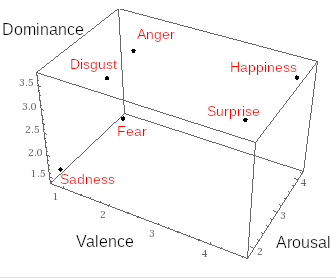
\includegraphics[scale=2]{litImgs/Ekmans3d.png}
\label{ekmans:graph}
\caption{3d plot of the figures given in Table \ref{ekmansTable}}
\end{figure}

